\documentclass[Analysis-3]{subfiles}

\begin{document}
\chapter*{Lecture 26} %Set chapter name
\addcontentsline{toc}{chapter}{Lecture 26} %Set chapter title
\setcounter{chapter}{26} %Set chapter counter
\setcounter{section}{0}

Recall \nameref{marker} discussed how to find area of a surface over a bounded region. Now we will look towards some example. 

\begin{Eg}{Truncated Cylinder}{}
    
    \begin{wrapfigure}{r}{0.50\textwidth}
        \centering
        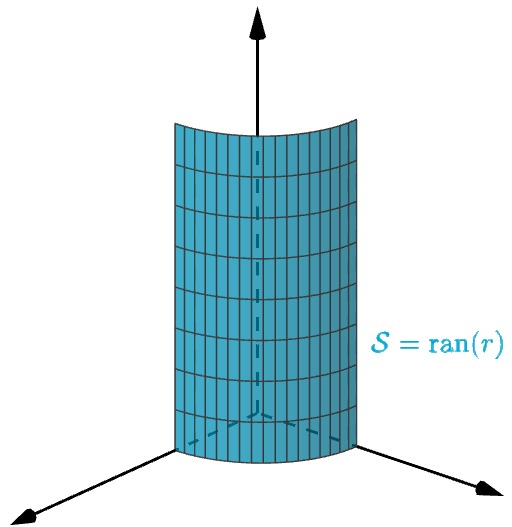
\includegraphics[width=.78\linewidth]{figures/lec-26.1.png}
        \caption{Truncated Cylinder}
    \end{wrapfigure}

 Let, $\mathcal{R} \subseteq \R^2$ be a region. $r : \mathcal{R} \to \R^3$ be a map defined by $r(x,y) = (\cos(x),\sin(x),y)$. Here the region is given by, 
\[\mathcal{R} = \{(x,y) | 0 \le x \le \frac{\pi}{2} , 0\le y \le 1\} = \qty[0,\frac{\pi}{2}] \times [0,1] \]

It can be seen easily that $r$ is parametrization of a surface $\text{ran}(r) = \mathcal{S}$. We want to calculate the surface area of it.

\textit{Area} of $\mathcal{S}$. For this case, $r_x = (-\sin x, \cos x, 0)$ and $r_y =(0,0,1)$. So, $ r_x \times r_y = (\cos x, \sin y,0)$ and 

\vspace{0.1cm}

hence $\norm{r_x \times r_y} = 1$.

\[\therefore \text{Area}(\mathcal{S}) = \int_{\mathcal{R}} 1 \dd A = \int_0^{\frac{\pi}{2}} \int_{0}^1 1 \dd A = \frac{\pi}{2}\]

\end{Eg}


\begin{Eg}{Hemisphere}{}
    
    \begin{wrapfigure}{r}{0.50\textwidth}
        \centering
        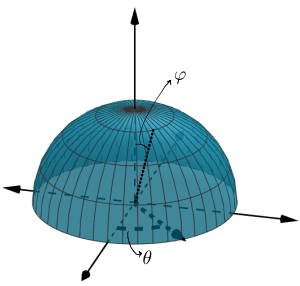
\includegraphics[width=.78\linewidth]{figures/lec-26.2.png}
        \caption{Hemisphere}
    \end{wrapfigure}

    $\mathcal{S} = \qty{(x,y,z) | x^2+y^2+z^2 = 1 , z >0 }$ is a surface. This surface actually surface of unit Hemisphere.
 
    parametrization of the surface $\mathcal{S}$ is given by, $r(\theta, \varphi) = (\cos \theta \cos \varphi, \sin \theta \cos \varphi , \sin \varphi)$ where, $0 \le \varphi \le \frac{\pi}{2} , 0 \le \theta \le 2\pi$.

    \begin{align*}
        \therefore r_{\theta} &= (-\sin \theta \cos \varphi, \cos \theta \cos \varphi, 0) \\
        r_{\varphi} &= (-\cos \theta \sin \varphi,-\sin \theta \sin \varphi , \cos \varphi) \\
        \therefore r_{\theta} \times r_{\varphi} &= (\cos \theta \cos ^2 \varphi, \sin \theta \cos ^2\varphi, \cos \varphi  \sin \varphi) \\
        \implies \norm{r_{\theta} \times r_{\varphi}} &= \cos \varphi 
    \end{align*}

    \[\text{Area}(\mathcal{S}) = \int_{0}^{\frac{\pi}{2}}\int_{0}^{2\pi} \cos \varphi \hspace{0.1cm} \dd \theta \dd \varphi = 2\pi \]

\end{Eg}

\section{Surface Integral over Scaler fields}

Let, $\mathcal{R} \in \R^2$ be a region. $r:\mathcal{R} \to \R^3$ be parametrization of a surface $\mathcal{S}$. $f$ be a scaler function defined on the surface $\mathcal{S}$. Let,$f \in C(\mathcal{S})$ then we can define integration of $f$ over the surface as following,

\begin{align*} 
    \int_{\mathcal{S}} f \hspace{0.1cm} \dd \mathcal{S} &:= \lim_{\norm{\mathcal{P}} \to 0} \sum_{\alpha \in \Lambda (\mathcal{P})} f(r(x_{\alpha})) \norm{r_u(x_{\alpha}) \times r_v(x_{\alpha})} \text{Area}(B_{\alpha}^2) \\
    &= \int_{\mathcal{R}} (f \circ r)(u,v) \norm{r_u \times r_v} \hspace{0.1cm} \dd A \cdots (*)
\end{align*}

As we have noticed in the case of \textbf{Line Integral of over a scaler field} the integration do not depend on the parametrization of the path. In this case also if we have different two parametrization $r,\tilde{r}$ for the surface $\mathcal{S}$ then there exist a one-one continus function $\varphi$ so tha the following diagramm commutes,(in other words $r = \tilde{r} \circ \tilde{\varphi}$)

\[\begin{tikzcd}
	& {\mathcal{S}} \\
	{\mathcal{R}} && {\tilde{\mathcal{R}}}
	\arrow["r", from=2-1, to=1-2]
	\arrow["{\tilde{r}}"', from=2-3, to=1-2]
	\arrow["\varphi"', from=2-1, to=2-3]
\end{tikzcd}\]
 
We can show that the integration in $(*)$ is also same if we replace $r$ by $\tilde{r}$. In other words the surface Integral over a surface is independent of it's parametrization.

\begin{Eg}{Surface Integral over a Cone}{}
We want to evaluate \[ \int_{\mathcal{S}}(x^2+y^2+z^2) \dd \mathcal{S}\]    

where, $\mathcal{S} = \qty{(x,y,z) | z = \sqrt{x^2 + y^2},0 \le z \le 1}$

\textit{Solution.} Let,$\mathcal{R} = \qty{(x,y)| x^2+y^2 \le 1}$ be the region and $r(x,y) = (x,y,\sqrt{x^2+y^2})$ is the parametrization of the surface $\mathcal{S}$. Here, $r_x = (1,0, \frac{x}{\sqrt{x^2+y^2}})$ and $r_y = (0,1,\frac{y}{\sqrt{x^2+y^2}})$.


\begin{align*}
    \therefore \int_{\mathcal{S}}(x^2+y^2+z^2) \dd \mathcal{S} &= \int_{\mathcal{R}} (f\circ r) \cdot \norm{r_x \times r_y} \dd A \\
    &= \int_{\mathcal{R}} (f\circ r) \sqrt{1 + \frac{x^2}{x^2+y^2} + \frac{y^2}{x^2+y^2}} \dd A \\
    &= 2\sqrt{2} \int_{\mathcal{R}} (x^2+y^2) \dd A \\
    &= 2\sqrt{2} \int_{0}^{1} \int_{0}^{2\pi} r^3 \hspace{0.1cm} \dd \theta \dd r \hspace{0.2cm} (\text{It's the polar substitution})\\
    &= \sqrt{2} \pi 
\end{align*}

\end{Eg}

\section{Surface Integral over a Vector field}

Let,$\vec{F} : \mathcal{S} \to \R^3$ be a vector field defined on a surface $\mathcal{S}$.We want to compute the extent to which $\vec{F}$ is pushing the surface along normal to $\mathcal{S}$.

%The content
\end{document}